
\begin{frame}[ctb!]
  \frametitle{Thermal Base Case Demonstration}
  \footnotesize{
A validation exercise comparing the combined scaling and  
superposition calculations demonstrates an average error of 1.1\% and a 
maximum error of 4.4\%,
\begin{figure}[htp!]
\begin{center}
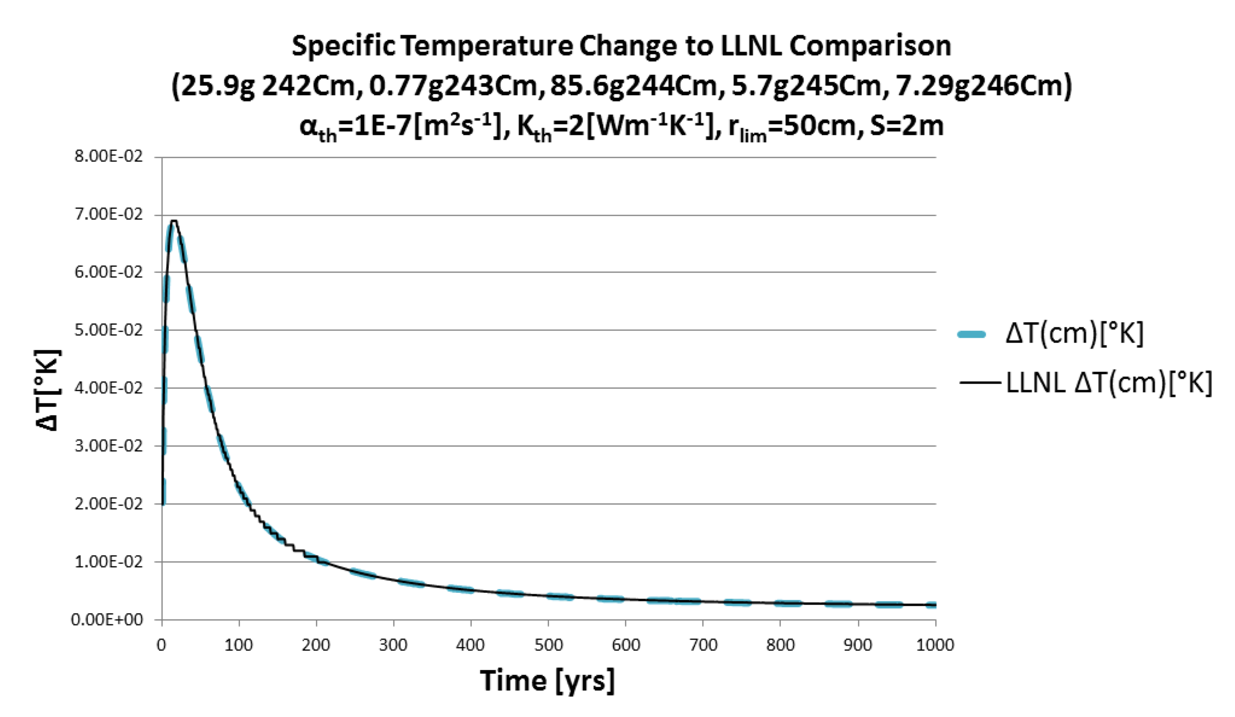
\includegraphics[width=\columnwidth]{./thermal_demonstration/CmValidation.eps}
\end{center}
\caption{This comparison of STC calculated thermal response from $Cm$ 
inventory per MTHM in 51GWd burnup UOX PWR fuel compares favorably with results 
from the semi-analytic model from LLNL.} 
\label{fig:CmValidation}
\end{figure}
  }
\end{frame}


\begin{frame}[ctb!]
  \frametitle{Thermal Base Case Demonstration}
Here, percent error is 
\begin{align}
\mbox{ percent error } &= 100\times\frac{\left|\Delta T_{LLNL} - \Delta 
T_{STC}\right|}{ \Delta T_{LLNL}}.
\end{align}
\begin{figure}[htp!]
\begin{center}
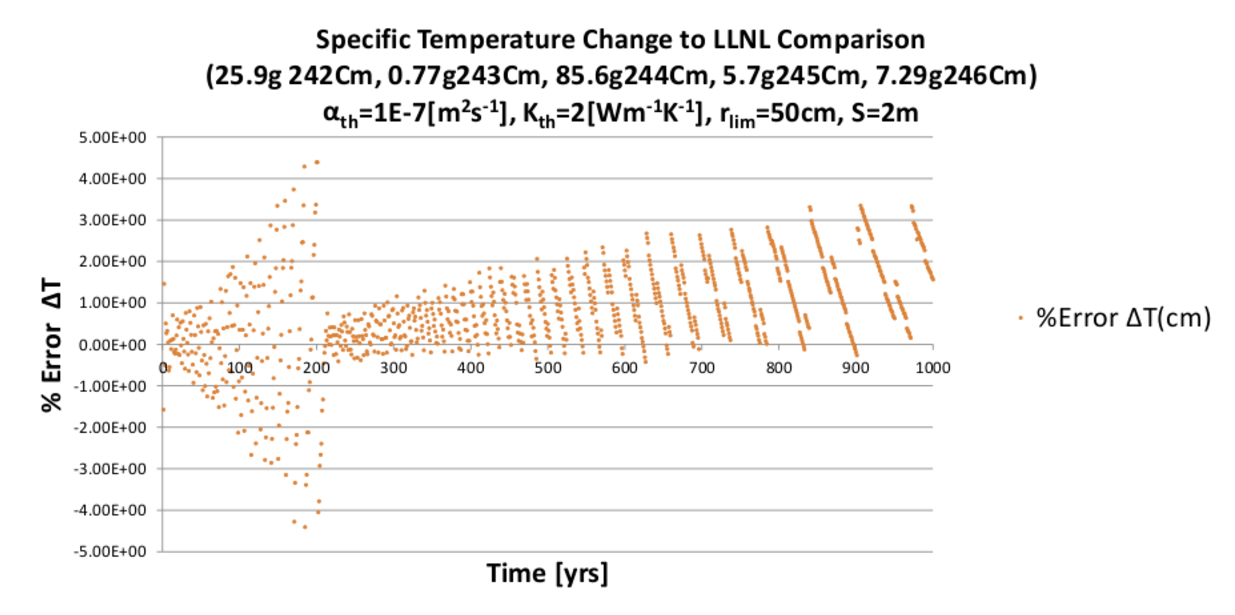
\includegraphics[width=\columnwidth]{./thermal_demonstration/CmPercentError.eps}
\end{center}
\caption{Percent error between the semi-analytic model from LLNL and the 
STC 
calculated thermal response from $Cm$ inventory per MTHM in 51GWd burnup UOX 
PWR fuel demonstrates a maximum percent error of 4.4\%.}
\label{fig:CmPercentError}
\end{figure}
\end{frame}

